\section{Introduction}

The terms ``vector'' and ``(one-dimensional) array'' appear so often as
synonyms that you may believe they actually are. In reality, computer
scientists and mathematicians mean different things by ``vectors''.  Computer
science is rife with terms such as ``vectorization'', ``vector machine,
``vector registers,'' and ``vector architecture'', where a ``vector''
simply means an ordered sequence of similar objects, or a one-dimensional
array. This meaning of ``vector'' is used in terms like ``vector operations''
to mean sorting, computing averages along an axis, and so on.
In contrast, mathematicians speak of ``vectors'' that are elements of
vector spaces. In the most abstract formulation, there is nothing said about
what the elements of a vector space are, only what operations are defined over
the vectors and the underlying scalar field.
In scientific computing, these two meanings of vectors can clash and cause
problems, particularly when working with matrices and vectors in the
conventions of numerical linear algebra in expressions like
$x^\prime Ay/x^\prime y$.

There are a few clues that a problem exists:


\begin{enumerate}

\item
Computer science terms like ``vectorization'' refer to one dimensional arrays
of homogeneous objects. Vectorized operations, like \code{sin(x)} for an array
\code{x}, have no need for the structure of a vector space.

\item
Programming language design issues regarding how to express linear algebra,
such as Julia's ``Taking vector transposes seriously''~\cite{julia4774} and
Python's ``A dedicated infix operator for matrix multiplication''~
\cite{numpy4351,Smith2014}, attract hundreds of comments from users expressing
a diversity of mutually incompatible opinions.

\item
Some computer languages cannot express identities familiar from linear algebra,
like $(ab')c = a(b'c)$ for vectors $a$, $b$ and $c$, using only multiplication
and transposition operations. Instead, the outer product $ab'$ must be written
as a call to a dedication function, such as
\code{numpy.outer}\cite{numpy.outer} in Python or
\code{Outer}\cite{Wolfram.Outer} in Mathematica.

\item
The original ``Matrix Laboratory''~\cite{Moler1980} had only
two-dimensional complex arrays, linear algebra, and broadcasting array
operations like \code{sin(x)}. All other functionality like sorting an array
were retrofit onto later versions of MATLAB, but every natural one dimensional
operation takes an optional \code{dim} argument to distinguish between
operations over rows from operations over columns. The default \code{dim}
choice occasionally risks confusion.

\item
The linear algebra literature can be classified by whether vectors
appear first (on or close to page 1) or whether matrices appear first.
In the former case, vectors live in a vector space; in the latter,
we have vectors that are matrices with one row or column.

\item
Programming languages do not consistently define what it means to transpose a vector. They can be classified by whether the result is the identity (a no-op), an error, a $1\times n$ matrix, or a value of a special row vector type.

\item
The scalar product $u^\prime v$ can be written as both \code{u.T @ v} and
\code{u @ v} in NumPy/Python; both produce a scalar. The analogous R code, \code{u\%*\%v}, produces a $1\times1$ matrix.

\item
A matrix times a vector is a vector, except in R, where the result of \code{A \%*\% b} is a matrix.

\item
A two dimensional array can be recursively defined is an array of arrays. A matrix cannot be defined recursively, but instead is a row vector of column vectors or a column vector of row vectors, never a row vector of row vectors or a column vector of column vectors.

\item
Matrix multiplication $C=AB$, is often defined in a first course in linear algebra as taking the scalar product of rows of $A$ with columns of $B$.
In MATLAB, we can express the computation of \code{C(i,j)} as \code{A(i,:)*B(:,j)}, but not with \code{u=A(i,:);v=B(:,j);u'v}, which returns an error.
In R, the analogous \code{A[i,] \%*\% B[,j]} returns a $1\times1$ matrix.
In NumPy/Python, the analogous \code{A[i-1,:] @ B[:,j-1]} returns a scalar.
Furthermore, this definition is sound for real matrices but is ambiguous for complex matrices and matrices over non-self-dual vector spaces.
The MATLAB code \code{dot(A(i,:),B(:,j))} returns the wrong answer for complex matrices.

\item
In the mathematical literature, $1\times 1$ matrices are often identified with scalars, and $n\times 1$ matrices are often identified with vectors. However, MATLAB is the only programming language used in scientific computing which makes these identifications. All other languages require users to convert between $1\times 1$ matrices and scalars, and $n\times 1$ matrices and vectors explicitly.

\end{enumerate}


These examples illustrate how computers have trouble with abstractions that humans, to a fault, are so good at overlooking. In fact, we did not initially think that this paper was actually worth writing, until we dug into the details. Decades after APL made multidimensional arrays first class objects, and MATLAB made Householder notation popular in computer code, we recently reached an inescapable conclusion, one we preferred not to believe, that vectors, in the sense of computer languages, and linear algebra vectors have serious coexistence issues.

The discrepancies listed above illustrates that computers struggle to identify quantities that humans treat as equivalent. The specific examples of quantities that humans treat as equivalent that most computer languages do not are:

\begin{itemize}
\item
Scalars, $1$-vectors, and $1\times1$ matrices. Each of these define scalar fields which can be used to define vector spaces over. However, most programming languages distinguish between these quantities, for example by providing different indexing behaviors.

\item
$n$-vectors, $1\times n$ matrices and and $n\times1$ matrices. All of these can be used as vectors in vector spaces that are all isomorphic to each other.

\end{itemize}

\begin{figure}
\caption{A menagerie of objects that one might not care to distinguish. Historically,
the distinction between column matrices and column vectors (and similarly
for rows) was not made until some time around the 1930s.}

\begin{centering}
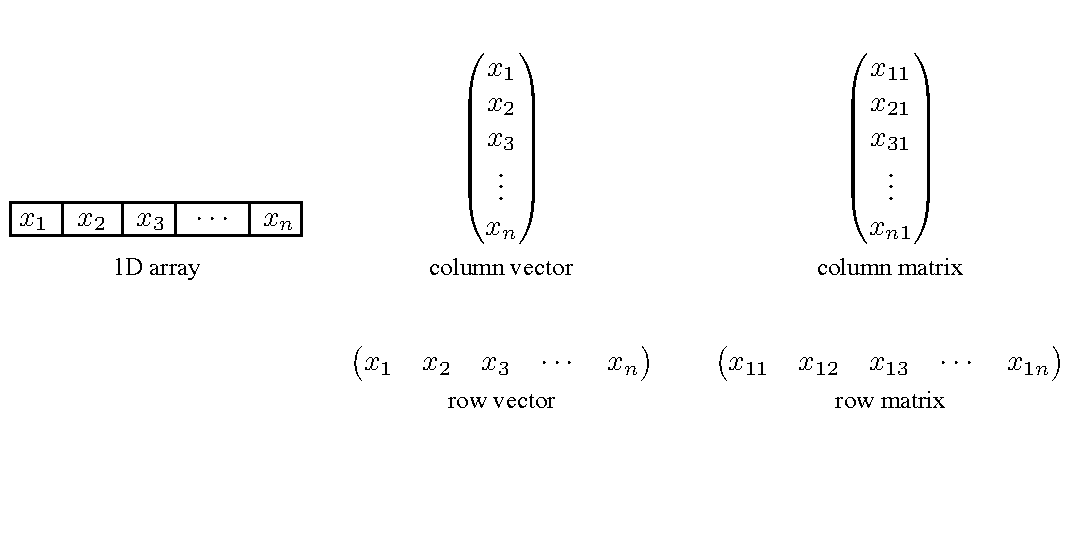
\includegraphics[width=0.95\columnwidth]{figures/fig-zoo}
\par\end{centering}
\end{figure}

For the purposes of this discussion, we use the following definitions.
\begin{description}
\item [{Definition}] An \textbf{array} or \textbf{one-dimensional} \textbf{array}
of size $N$ is a collection of elements $F$ and an indexing function
$idx:\left\{ 1,2,\dots,N\right\} \mapsto F$ that allows the getting
and setting of the $i$th element.
\item [{Definition}] A \textbf{matrix} is a two-dimensional array of size
$M\times N$, i.e. it is a collection of elements $F$ and an indexing
function $idx:\{\left(1,1\right),\left(1,2\right),\dots,\left(1,N\right),\left(2,1\right),\left(2,2\right),\dots,$
$\left(2,N\right),\dots,\left(M,N\right)\}\mapsto F$ that allows
the getting and setting of the $\left(i,j\right)$th element.
\item [{Definition}] A \textbf{vector} is an ordered tuple of $N$ scalars
from a field $F$ that is an element of a vector space $F^{N}$.
\end{description}
From the first definition, we get indexing behavior. From the second
defition, we get algebra, i.e. a defined interface of what operations
like addition $+$ and multiplication $*$ mean.

The problem arises when considering this alternate definition of a
vector:
\begin{description}
\item [{Definition}] A \textbf{column vector} is a column matrix, i.e.
a matrix with one column. A \textbf{row vector} is a row matrix, i.e.
a matrix with one row.
\end{description}
In this latter definition, vectors have intrinsic rowness or columnness.
In the former definition, vectors are intrinsically flat and have
no notion of rowness or columnness.

Figure 1 shows

and transposition $\prime$All languages can be divided into languages
that retrofitted linear algebra onto arrays, or else grafted array
semantics onto linear algebra.

Computer science talks about arrays; mathematics talks about vectors
and matrices. As data structures, we want indexing behavior. As linear
algebraic objects, we want algebra, i.e. a defined interface of $+,*,'$.

Thesis: one-dimensional arrays have fundamenatally different semantics
from vectors.

Consider only fixed size arrays for now. The problem now shows up
when asking about what the transpose of a vector should be. A 1-D
array by definition can be indexed with a single subscript, $A[i]$,
and has shape $\left(n,\right)$. In contrast, vectors in linear algebra
are often assumed to have intrinsic rowness or columnness. For example,
an expression like the bilinear form $x^{T}Ay$ is thought of as the
product of $x^{T}$, $A$ and $y$. While $x^{T}$ and $y$ are usually
considered vectors, the former is a row vector whereas the latter
is a column vector. They have fundamentally different algebras: $y$
can only be premultiplied by a matrix $A$ of conformant shape, and
$x^{T}$ can only be postmultiplied.

\begin{figure}
\caption{Flat vectors vs row/column vectors and embeddings and transpositions.}

\centering{}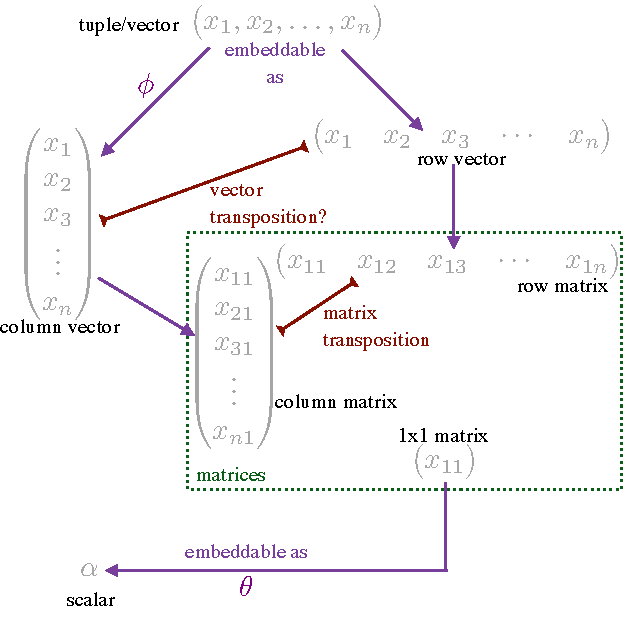
\includegraphics[width=0.9\columnwidth]{figures/fig-embed}
\end{figure}

Isomorphisms between these various quantities are ubiquitous in the mathematical literature of linear algebra, but are rare, if outright nonexistent, in computer science. The former is used to expressions written in Householder notation~\cite{Householder1953,Householder1955} like $x^\prime Ay/x^\prime y$; in Sec.~\ref{sec:householder}, we discuss explicitly the embeddings used in expressions like inner products $u^T v$, outer products $u v^T$, and bilinear forms $u^T A v$. In Sec.~\ref{sec:math_history}, we review the historical development of matrices and vectors in linear algebra, demonstrating that the modern presentation of matrices and vectors has a surprisingly recent history. The latter studies indexing, mapping and reduction operations, like sorting and computing means along axes. Because of the fundamentally incompatible disagreements of which quantities to treat as equivalent, we argue in this paper that it is impossible to have our beloved Householder notation and one dimensional arrays in the same language without some sort of compromise. In Sec.~\ref{sec:array}, we review how arrays are used in computer science and review their history in Sec.~\ref{sec:array_history}. Finally, we review in Sec.~\ref{sec:reallanguages} how array and vector semantics are implemented in various languages.
